\documentclass[11pt,a4paper]{article}

\usepackage[utf8]{inputenc}
\usepackage[T1]{fontenc}
\usepackage[portuguese]{babel}
\usepackage{amsmath}
\usepackage{amsfonts}
\usepackage{graphicx}
\usepackage{geometry}
\usepackage{xcolor}
\usepackage{booktabs}
\usepackage{hyperref}
\usepackage{listings}

\geometry{left=2.5cm, right=2.5cm, top=3cm, bottom=3cm}

% --- Configuração para exibição de código Python ---
\definecolor{codegreen}{rgb}{0,0.6,0}
\definecolor{codegray}{rgb}{0.5,0.5,0.5}
\definecolor{codepurple}{rgb}{0.58,0,0.82}
\definecolor{backcolour}{rgb}{0.95,0.95,0.92}

\lstdefinestyle{mystyle}{
    backgroundcolor=\color{backcolour},   
    commentstyle=\color{codegreen}\bfseries,
    keywordstyle=\color{blue},
    numberstyle=\tiny\color{codegray},
    stringstyle=\color{codepurple},
    basicstyle=\ttfamily\footnotesize,
    breakatwhitespace=false,         
    breaklines=true,                 
    captionpos=b,                    
    keepspaces=true,                 
    numbers=left,                    
    numbersep=5pt,                  
    showspaces=false,                
    showstringspaces=false,
    showtabs=false,                  
    tabsize=4
}
\lstset{style=mystyle}

\title{\textbf{Relatório Técnico - Crédito 2}\\
\Large{Determinação Experimental da Complexidade de Tempo do FCM}}
\author{\textbf{Equipe 10 -- Anti-team}\\
Missão 4 -- Loop Unrolling (Força Bruta)\\
\small Rafael Souza Santana -- 072410098\\
\small Felipe dos Santos -- 072120189\\
\small Luiz Carlos dos Santos Ferreira Sacramento -- 071820393\\
\small Auditoria cruzada: Equipe 2 -- Pixely\\
\small Universidade do Estado da Bahia (UNEB) -- DCET I}
\date{29 de outubro de 2026}
\begin{document}
\maketitle

\section{Introdução e Escopo}
Este trabalho investiga o tempo de execução do Fuzzy C-Means (FCM) em função
do número de pixels $n$ e do número de grupos $K$. A Equipe 10 -- Anti-team
é responsável pela \textbf{Missão 4 -- Loop Unrolling (Força Bruta)}:
desenrolar somente os pequenos laços que percorrem os três canais RGB,
conforme o mapa cirúrgico da disciplina \cite{missao,template}.

O ponto de partida é o código oficial do professor \cite{base}. O objetivo
é verificar se a mudança na organização desses laços preserva os resultados
e altera o tempo de processamento. A comparação usa as mesmas entradas,
parâmetros e inicialização nas duas versões. O trabalho também apresenta a
integração do FCM Puro ao notebook experimentador utilizado em sala.

\subsection{Como o FCM representa os grupos}
No K-Means, cada pixel pertence a um único grupo. No FCM, um mesmo pixel pode
ter diferentes graus de pertinência. Esses valores formam a matriz
$U\in[0,1]^{n\times K}$: $u_{ij}$ indica a participação do pixel $i$ no grupo
$j$, com $\sum_{j=1}^{K}u_{ij}=1$ em cada linha.
Essa representação permite descrever pixels próximos da fronteira entre grupos.

Cada pixel é um vetor $x_i=[R,G,B]$, e cada grupo tem um centroide $c_j$ com
três coordenadas. A função objetivo do FCM pondera as distâncias pelas
pertinências:
\begin{equation}
 J_m(U,C)=\sum_{i=1}^{n}\sum_{j=1}^{K}u_{ij}^{m}\lVert x_i-c_j\rVert^2.
\end{equation}
O parâmetro $m>1$ controla a distribuição das pertinências; nos experimentos,
$m=2$. Os centroides são atualizados por médias ponderadas:
\begin{equation}
 c_j=\frac{\sum_{i=1}^{n}u_{ij}^{m}x_i}{\sum_{i=1}^{n}u_{ij}^{m}}.
\end{equation}
Para distâncias não nulas, a atualização das pertinências é
\begin{equation}
 u_{ij}=\left[\sum_{\ell=1}^{K}
 \left(\frac{\lVert x_i-c_j\rVert}{\lVert x_i-c_{\ell}\rVert}\right)^{2/(m-1)}
 \right]^{-1}.
\end{equation}
Assim, o algoritmo começa com $U$ aleatória e normalizada; recalcula os
centroides; calcula as distâncias e as novas pertinências; e verifica a maior
mudança $\Delta U$. O ciclo termina quando $\Delta U<\epsilon$ ou quando o
limite de iterações é atingido. O tratamento de distâncias nulas é o do
baseline, cujas limitações são descritas na seção de validação.

\section{Análise da Restrição Arquitetural}
\textbf{Restrição sorteada: Missão 4 -- Loop Unrolling.}
No baseline, \texttt{for c in range(canais)} executa o mesmo corpo para cada
canal. Com entrada RGB, os índices são sempre 0, 1 e 2. A variante escreve
as três operações explicitamente, mantendo sua ordem e os mesmos valores.
A Tabela~\ref{tab:alvos} localiza as únicas intervenções.

\begin{table}[htbp]\centering\small
\caption{Mapa das três alterações no baseline oficial.}\label{tab:alvos}
\begin{tabular}{@{}lp{7.1cm}r@{}}\toprule
Trecho & Operação mantida no corpo & Linhas originais\\\midrule
Acumulação do centroide & Somar $u_{ij}^{m}x_i$ em cada canal do numerador & 43--44\\
Montagem do centroide & Dividir cada coordenada pelo denominador & 47--48\\
Distância RGB & Somar os quadrados das diferenças de cada canal & 61--63\\
\bottomrule\end{tabular}
\end{table}

Os laços de pixels, grupos e convergência permanecem iguais. As fórmulas,
a estrutura de listas e o critério de parada também permanecem.
Não é necessário tratar resto de divisão: os três canais são totalmente
desenrolados. O adaptador exige RGB antes da medição; não se desenrolam
pixels nem se fixa o número de grupos no núcleo.

\subsection{Relação com F.O.C.A. e hardware}
O anexo descreve a taxa de gestão de laço $o+c+4a$, associada a operação,
comparação e atribuições \cite{missao}. O desenrolamento retira a gestão dos
pequenos laços, mas preserva as multiplicações, divisões e acessos RGB de seus
corpos. Se $I$ for o número de iterações principais executadas, os três pontos
da Tabela~\ref{tab:alvos} são acionados $InK$, $IK$ e $InK$ vezes,
respectivamente. Portanto, há $2InK+IK$ ocorrências desses pequenos laços
na execução original. Essa localização prepara a contagem completa do Crédito 3.

A contrapartida proposta pela missão é trocar saltos e avaliações de laço
por mais instruções explícitas, com possível efeito na memória de instruções
(I-Cache). Em CPython, o interpretador e o acesso a objetos também participam
do custo. A bancada mede tempo de parede; não utiliza contadores de I-Cache
ou pipeline. Assim, um ganho medido não identifica, sozinho, qual desses
mecanismos foi responsável pela diferença.

\section{Implementação do Núcleo FCM}
O baseline está em \texttt{src/fcm\_baseline.py}; a variante está em
\texttt{src/fcm\_unrolling.py}. O diff da missão registra as três substituições.
O repositório reúne código-fonte, testes, experimentador, entradas, dados reais
e instruções de reprodução. \textbf{Repositório público:} \href{https://github.com/rssantan4/UniSolves/tree/main/EngenariadeProgramas/FCM_Credito2_Missao4}{rssantan4/UniSolves -- FCM Crédito 2}.

O trecho abaixo mostra os blocos alterados, dentro dos respectivos laços
originais. As demais fases do FCM não foram refatoradas.

\noindent\begin{minipage}{\linewidth}
\begin{lstlisting}[language=Python,caption={Operações RGB explícitas na variante.}]
# 1. Dentro da acumulacao do centroide (lacos j e i)
numerador[0] += u_m * X[i][0]
numerador[1] += u_m * X[i][1]
numerador[2] += u_m * X[i][2]

# 2. Montagem do centroide (dentro do laco j)
centroide_j.append(numerador[0] / denominador)
centroide_j.append(numerador[1] / denominador)
centroide_j.append(numerador[2] / denominador)

# 3. Distancia RGB (dentro dos lacos i e j)
diff = X[i][0] - C[j][0]
soma_quadrados += diff * diff
diff = X[i][1] - C[j][1]
soma_quadrados += diff * diff
diff = X[i][2] - C[j][2]
soma_quadrados += diff * diff
\end{lstlisting}
\end{minipage}

\subsection{Validação funcional}
Os \textbf{12 testes} foram aprovados: cinco verificam equivalência e estrutura
do núcleo, quatro verificam as fontes de imagem e três auditam os resultados
estatísticos. A comparação estrutural exige exatamente a expansão dos três
laços RGB. Nos casos funcionais, verificam-se centroides, matriz $U$,
trajetória de convergência, finitude dos valores, soma das pertinências e
preservação da entrada.

Na demonstração com a fonte I1, $n=1024$, $K=3$ e seed 42, as duas versões
executaram 12 iterações e terminaram com $\Delta U\approx0{,}008026$.
As maiores diferenças entre centroides e entre pertinências foram zero.
Essa execução é funcional, realizada fora da coleta de tempos.
Por exemplo, um pixel da demonstração teve pertinências aproximadas
$[0{,}482;\,0{,}033;\,0{,}485]$: ele é quase igualmente associado aos grupos
0 e 2, informação que uma única classificação rígida esconderia.

As singularidades herdadas não foram corrigidas: o código pode dividir por
zero quando uma distância nula ocorre em um centroide posterior e pode
encerrar a verificação da variação de $U$ de forma incompleta nesse caso.
Os testes reproduzem essas limitações nas duas versões; elas não resultam
do Unrolling.

\subsection{Exemplo visual da segmentação}
Para visualizar o resultado, cada pixel recebe a cor do centroide cujo grau
de pertinência é maior ($\arg\max U$). Essa reconstrução é feita depois do
FCM, fora do cronômetro, e não modifica o núcleo. A Figura~\ref{fig:segmentacao}
reutiliza uma saída salva do notebook Puro. O exemplo ajuda a interpretar
os grupos, mas não é uma avaliação da qualidade da segmentação.
\begin{figure}[htbp]\centering
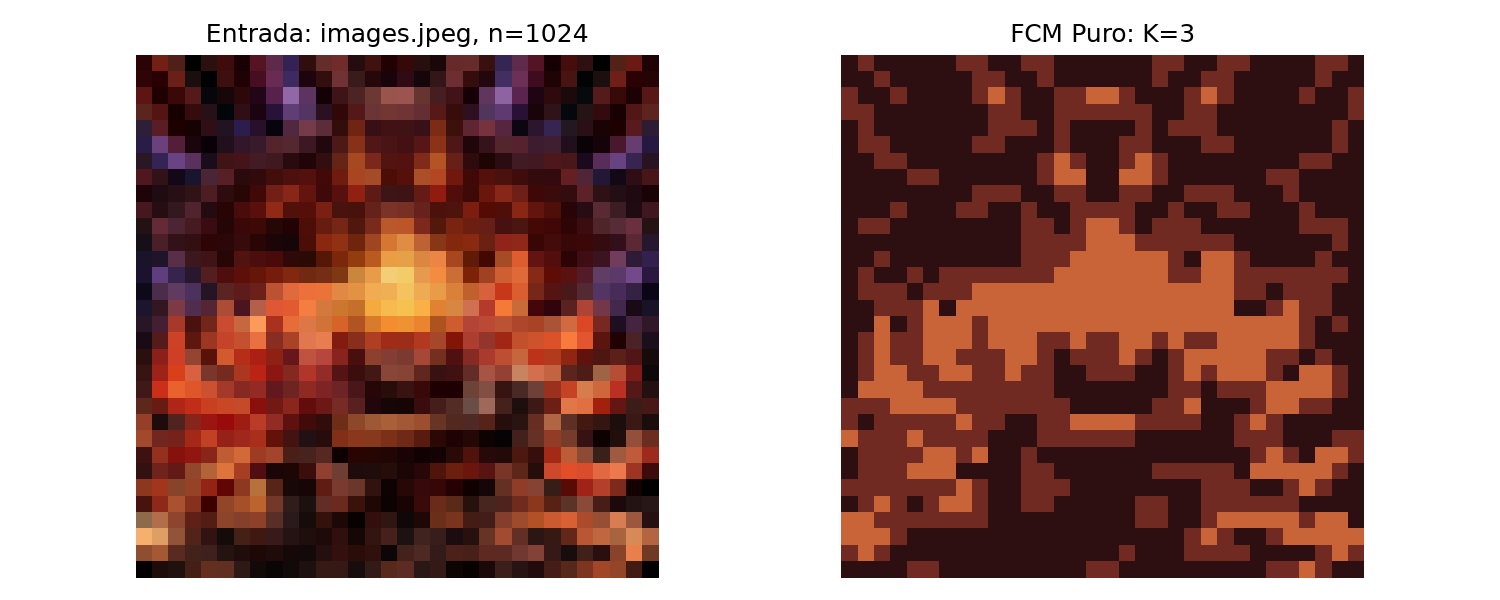
\includegraphics[width=0.88\linewidth]{exemplo_segmentacao.png}
\caption{Fonte I1, $32\times32$ pixels e $K=3$: entrada e segmentação pelo FCM
Puro, extraídas da coleta N. A baixa resolução faz parte da malha experimental.}
\label{fig:segmentacao}
\end{figure}

\section{Metodologia Experimental e Estabilidade}
\subsection{Entradas e parâmetros}
As fontes são I1: \texttt{images.jpeg}, I2: \texttt{images (1).jpeg} e
I3: \texttt{images (2).jpeg}, com dimensões originais $480\times640$,
$597\times335$ e $385\times519$, respectivamente.
Cada fonte foi convertida para RGB e redimensionada com LANCZOS para lados
16, 24, 32, 48 e 64. Logo,
$n\in\{256,576,1024,2304,4096\}$, com $K\in\{2,3,4\}$.
Os redimensionamentos são entradas derivadas, não novas fontes independentes.
O formato quadrado altera as proporções; o interesse é controlar o tamanho
computacional, não preservar a aparência da imagem original.

Usaram-se $m=2$, $\epsilon=0{,}01$, máximo de 100 iterações, seed 42 e
$R=30$ repetições por caso, conforme o template. Reaplicar a mesma seed
controla a inicialização na comparação; não representa um estudo de
sensibilidade a diferentes sementes.

\subsection{Duas coletas identificadas}
\begin{itemize}
\item \textbf{C -- comparação da Missão 4:} fontes I1 e I2, baseline e
Unrolling; $2\times5\times3\times2\times30=1.800$ tempos.
A ordem das duas versões alterna entre repetições, e cada caso tem aquecimento.
O GC padrão do Python foi mantido. Resultado: \textbf{58/60 séries homologadas}.
\item \textbf{N -- notebook FCM Puro:} fontes I1, I2 e I3, apenas baseline;
$3\times5\times3\times30=1.350$ tempos.
Antes de cada medição, as saídas anteriores são liberadas, executa-se
\texttt{gc.collect()} e a seed é reaplicada; o GC automático continua ativo
durante o FCM. Resultado: \textbf{45/45 séries homologadas}.
\end{itemize}

A coleta C foi feita por \texttt{experimentador.py}. A coleta N foi executada
no notebook integrado, em kernel Jupyter local utilizado pelo VS Code.
Ambos derivam do experimentador do professor e mantêm
\texttt{perf\_counter()}, filtragem P5--P95, estatísticas, ajuste e gráficos.
O timer envolve a chamada completa do FCM, desde a inicialização de $U$
até o retorno. Leitura, conversão para listas RGB, seed, aquecimento,
exportação, impressões e gráficos ficam fora desse intervalo.

A máquina foi Apple M4, 16 GiB, macOS 27.0.1, CPython 3.14.7.
As versões das dependências e os parâmetros estão nos arquivos de ambiente.
Energia e isolamento de processos concorrentes não foram aferidos.
A diferença de preparo entre C e N impede usar seus tempos como uma única
comparação Puro versus Unrolling. A terceira fonte não foi medida com a variante.

\subsection{O que significa homologar uma série}
Cada série reúne 30 tempos da mesma fonte, versão, $n$ e $K$.
O filtro retém os valores entre os percentis 5 e 95, inclusive. Os tempos
originais permanecem nos CSVs; o filtro não apaga medições.
Para os $r$ valores retidos, calculam-se
\[
 \bar t=\frac{1}{r}\sum_{i=1}^{r}t_i,\qquad
 s=\sqrt{\frac{\sum_{i=1}^{r}(t_i-\bar t)^2}{r-1}},\qquad
 CV=\frac{s}{\bar t}.
\]
O CV compara a dispersão com a média: por exemplo, $CV=0{,}02$ corresponde
a um desvio de 2\% da média. A regra é estrita: $CV<0{,}15$;
um valor igual a 0,15 reprovaria. Nestas coletas, 26 de 30 tempos foram
retidos em cada série. A Tabela~\ref{tab:cv} resume casos e inclui as duas
reprovações da comparação C; todas as combinações estão nos CSVs.
\begin{table}[htbp]\centering\footnotesize
\caption{Amostra de estabilidade. CVs reprovados em negrito.}
\label{tab:cv}
\begin{tabular}{@{}cclrrrrr@{}}\toprule
Coleta & Fonte & Versão & $n$ & $K$ & Média (s) & Desvio (s) & CV\\\midrule
C & 1 & Puro & 2304 & 2 & 0,028107 & 0,004703 & \textbf{0,167324} \\
C & 1 & Unrolling & 2304 & 2 & 0,023680 & 0,000101 & 0,004251 \\
C & 2 & Puro & 2304 & 2 & 0,026819 & 0,000152 & 0,005662 \\
C & 2 & Unrolling & 2304 & 2 & 0,026567 & 0,005973 & \textbf{0,224842} \\
N & 1 & Puro & 4096 & 4 & 0,266642 & 0,000664 & 0,002490 \\
N & 2 & Puro & 4096 & 4 & 0,213413 & 0,000847 & 0,003970 \\
N & 3 & Puro & 4096 & 4 & 0,204385 & 0,001735 & 0,008491 \\
\bottomrule\end{tabular}
\end{table}

A falha da fonte I1 é do baseline, com $CV=0{,}167324$; a da fonte I2 é da
variante, com $CV=0{,}224842$, ambas em $n=2304$, $K=2$.
A causa dos picos de tempo não foi estabelecida. O maior CV da coleta N foi
0,019384, mas essa aprovação não substitui as falhas de C, pois N não mediu
Unrolling e usa outro preparo. A homologação integral da missão exige nova
coleta válida sob condições equivalentes, preservando os tempos anteriores.


\section{Resultados Empíricos (\texorpdfstring{$T_{exp}$}{Texp})}
\subsection{FCM Puro: gráficos obrigatórios da bancada}
A coleta N executou o FCM Puro sem a intervenção Loop Unrolling, com as
três fontes de imagem, cinco tamanhos e $K\in\{2,3,4\}$, totalizando 45
séries com $R=30$. Todas tiveram $CV<0{,}15$, com máximo de $0{,}019384$.
A Figura~\ref{fig:baseline_graficos} apresenta os cortes $T\times n$ e
$T\times K$ e a superfície de tempo para a fonte I1. Os gráficos correspondentes
às fontes I2 e I3, os dados brutos e as tabelas completas estão disponíveis
no repositório, em \texttt{resultados/fcm\_puro\_notebook/}.
A coleta N foi realizada no notebook experimentador adaptado do material
oficial, e não deve ser confundida com o protocolo comparativo C.

\begin{figure}[htbp]\centering
\includegraphics[width=0.96\linewidth]{fcm_puro_imagem_01_2d.png}\\[0.5em]
\includegraphics[width=0.65\linewidth]{fcm_puro_imagem_01_3d.png}
\caption{FCM Puro, fonte I1: cortes bidimensionais do tempo de execução e
superfície $T_{exp}(n,K)$, obtidos na coleta N (homologada).}
\label{fig:baseline_graficos}
\end{figure}


\subsection{Função de tempo ajustada}
O modelo do template \cite{template} foi ajustado com \texttt{curve\_fit},
separadamente para cada fonte e versão:
\begin{equation}
 T_{exp}(n,K)=\alpha nK+\beta n+\gamma K+\delta.
\end{equation}
Os coeficientes descrevem a relação observada entre entrada e tempo.
O $R^2$ resume quanto o ajuste acompanha as médias medidas; ele não é uma
medida de qualidade da segmentação. A Tabela~\ref{tab:modelos} apresenta os
quatro ajustes da coleta C. O asterisco marca os que incluem série com CV
reprovado e, portanto, são exploratórios.
\begin{table}[htbp]\centering\footnotesize
\caption{Coeficientes da coleta C e qualidade do ajuste.}
\label{tab:modelos}
\begin{tabular}{@{}lrrrrr@{}}\toprule
Fonte/versão & $\alpha$ & $\beta$ & $\gamma$ & $\delta$ & $R^2$\\\midrule
I1/Puro * & 2.6077e-05 & -4.1397e-05 & -5.2580e-03 & 9.9241e-03 & 0,9675 \\
I1/Unrolling & 2.4243e-05 & -3.9302e-05 & -5.0301e-03 & 9.7181e-03 & 0,9676 \\
I2/Puro & 2.2860e-05 & -3.5630e-05 & -2.5578e-03 & 2.9539e-03 & 0,9371 \\
I2/Unrolling * & 2.0778e-05 & -3.2307e-05 & -2.4621e-03 & 2.9957e-03 & 0,9339 \\
\bottomrule\end{tabular}
\end{table}

Para a variante na fonte I1, a equação obtida, em segundos, é:
\[
 T_{exp}(n,K)=(2{,}424336\!\times\!10^{-5})nK
 -(3{,}930178\!\times\!10^{-5})n
 -(5{,}030144\!\times\!10^{-3})K+9{,}718082\!\times\!10^{-3}.
\]
As Figuras~\ref{fig:2d} e~\ref{fig:3d} mostram esse mesmo caso, cujas
15 séries passaram no CV. Os cortes 2D permitem observar o efeito de variar
$n$ com $K$ fixo e de variar $K$ com $n$ fixo. A superfície reúne as duas
variáveis; a distância dos pontos à superfície mostra que o ajuste não
reproduz exatamente todas as médias. Os PNGs são os originais da coleta.

Os coeficientes negativos não significam que existam etapas com tempo negativo:
eles fazem parte de um ajuste conjunto na malha estudada. O modelo não deve
ser extrapolado para tamanhos arbitrários. Além disso, o número efetivo de
iterações $I$ varia com a entrada e a convergência, o que ajuda a explicar
por que as médias não seguem uma função simples perfeitamente.

\begin{figure}[htbp]\centering
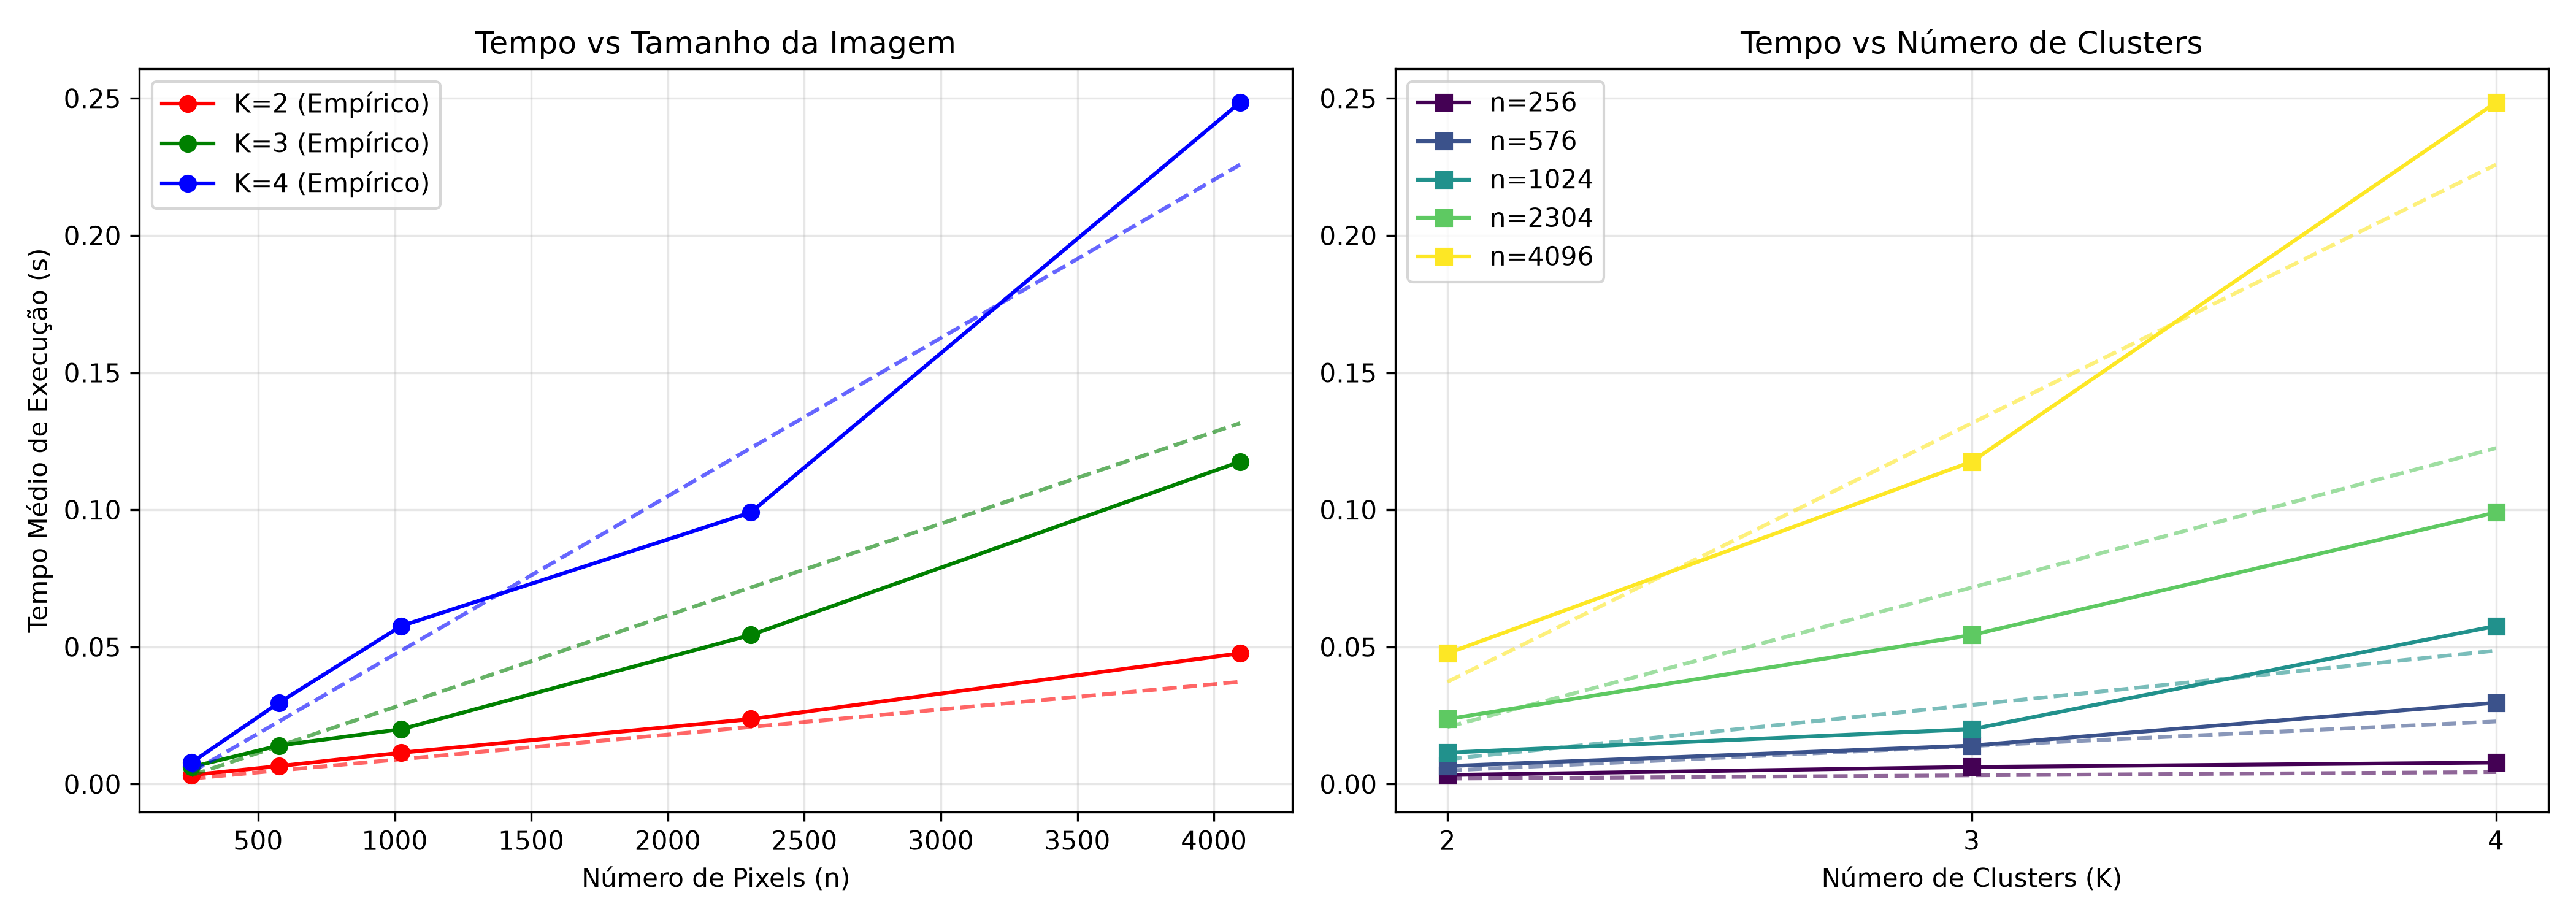
\includegraphics[width=\linewidth]{imagem_01_unrolling_relatorio_complexidade.png}
\caption{Missão 4, fonte I1: tempo $\times n$ e tempo $\times K$. Linhas
contínuas representam as médias medidas; tracejadas, o ajuste.}\label{fig:2d}
\end{figure}
\begin{figure}[htbp]\centering
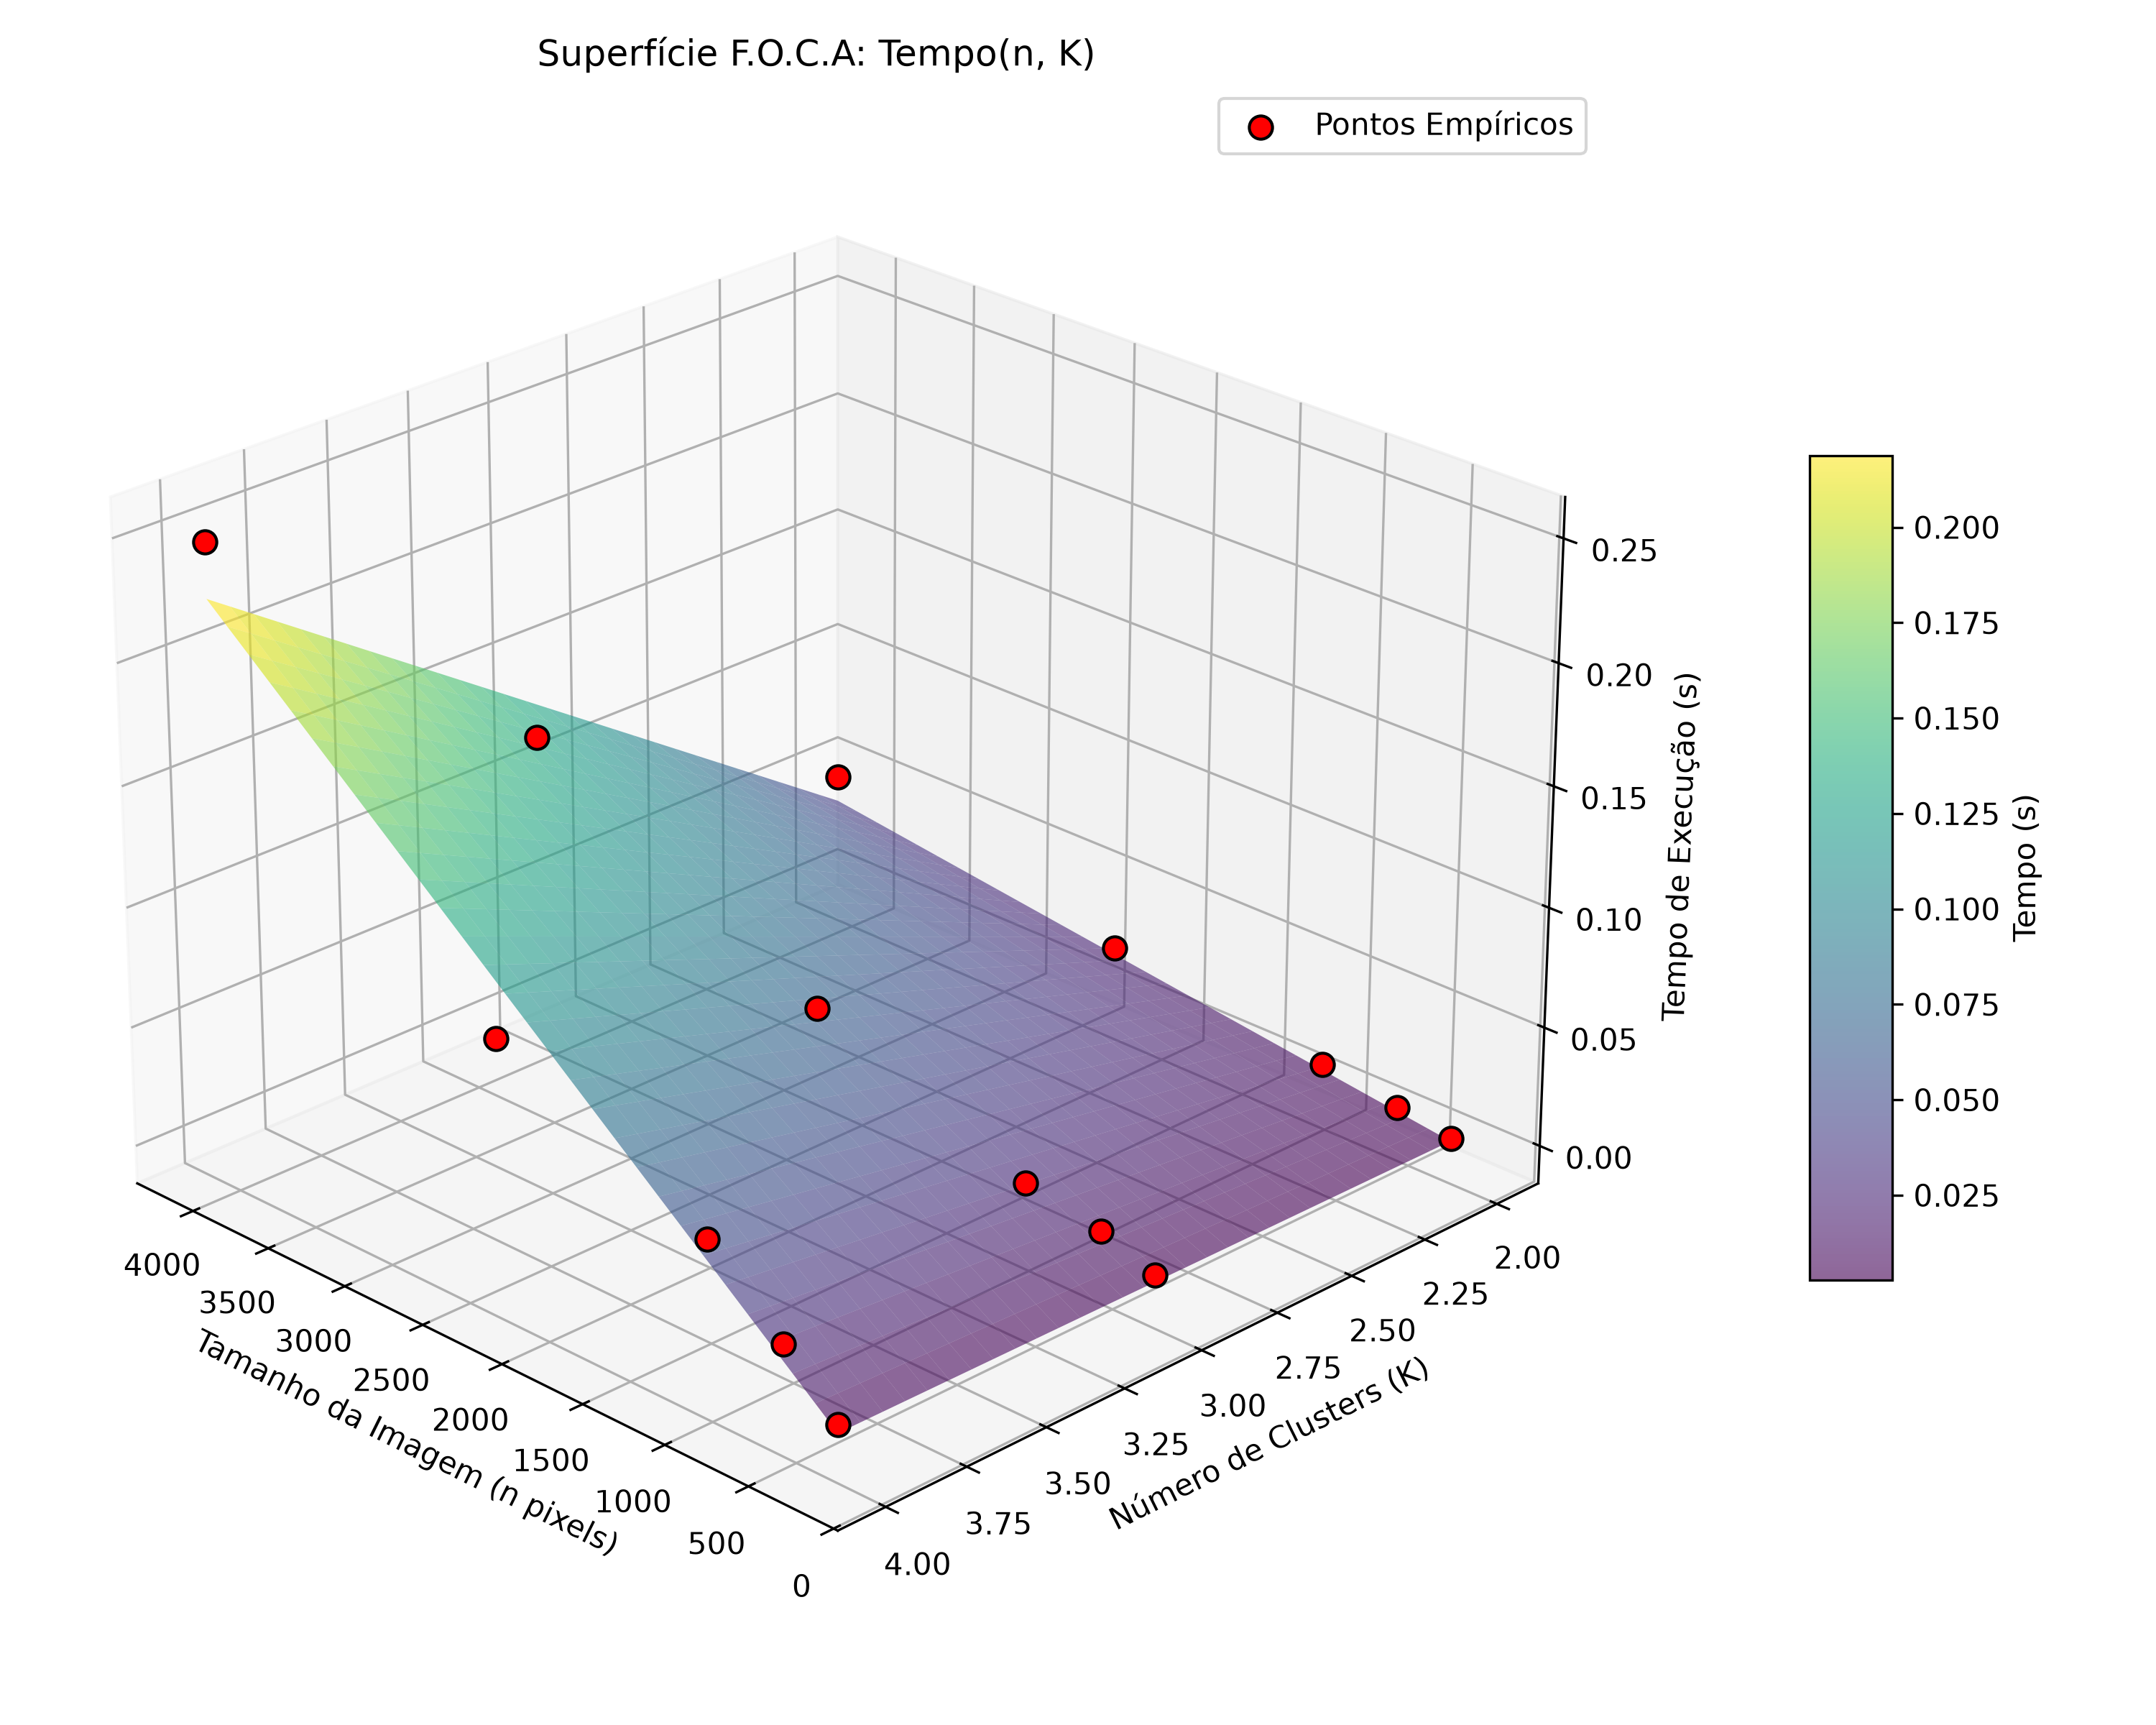
\includegraphics[width=0.82\linewidth]{imagem_01_unrolling_superficie_3d_foca.png}
\caption{Missão 4, fonte I1: superfície ajustada e pontos experimentais.}
\label{fig:3d}
\end{figure}

\subsection{Comparação entre baseline e Unrolling}
Para cada par medido sob o mesmo protocolo C, calcularam-se o quociente de
médias e a redução percentual:
\[
 S=\frac{\bar t_{puro}}{\bar t_{unrolling}},\qquad
 \text{redução}=100\left(1-\frac{\bar t_{unrolling}}{\bar t_{puro}}\right).
\]
Quando $S>1$, a variante tem menor tempo médio. A Tabela~\ref{tab:ganho}
resume somente os pares em que ambas as séries passaram no CV.
\begin{table}[htbp]\centering\small
\caption{Desempenho nos pares homologados da coleta C.}\label{tab:ganho}
\begin{tabular}{@{}lrrr@{}}\toprule
Fonte & Pares homologados & Redução (\%) & $S$\\\midrule
I1 & 14/15 & 8,39 a 12,77 & 1,092 a 1,146 \\
I2 & 14/15 & 8,44 a 11,23 & 1,092 a 1,127 \\
\bottomrule\end{tabular}
\end{table}

No conjunto desses 28 pares, a redução variou de 8,39\% a 12,77\%.
A Figura~\ref{fig:comparacao} mostra a comparação da fonte I1; a cruz vermelha
mantém visível o par com falha de CV. O gráfico da fonte I2 e as tabelas
completas permanecem nos resultados. Os dois pares não homologados não
entram na faixa de redução acima.
\begin{figure}[htbp]\centering
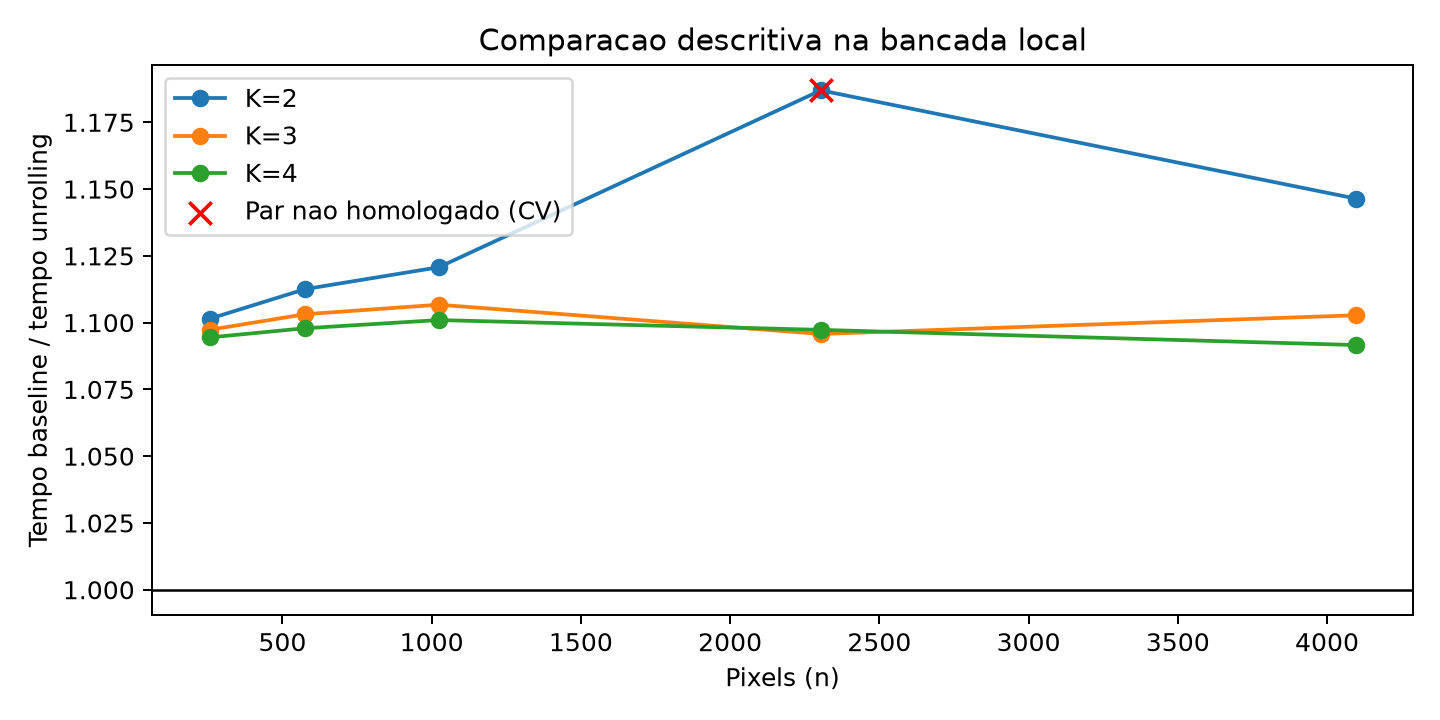
\includegraphics[width=0.95\linewidth]{imagem_01_comparacao.png}
\caption{Fonte I1: comparação de médias e aceleração relativa.
A marca vermelha identifica o par não homologado.}\label{fig:comparacao}
\end{figure}

Esse ganho é descritivo das entradas, parâmetros e máquina utilizados.
Não foi realizado teste de significância, e os dados não garantem melhoria
em outras imagens, sementes ou plataformas. CV baixo indica repetibilidade;
não demonstra, por si só, adequação do modelo ou causalidade de hardware.

\clearpage
\section{Conclusão Parcial}
A Equipe 10 implementou a Missão 4 com três expansões RGB, mantendo o restante
do FCM oficial. Os testes e a demonstração com inicialização controlada
preservaram centroides, pertinências e convergência. Na comparação existente,
a variante apresentou menor tempo médio nos 28 pares homologados, com redução
observada de 8,39\% a 12,77\%. Duas séries ainda não cumprem o critério de CV.
A coleta adicional do FCM Puro no notebook passou nas 45 séries das três fontes.

O modelo $\alpha nK+\beta n+\gamma K+\delta$ resume a malha experimental,
mas não prova $O(nK)$ para o algoritmo completo. A atualização de pertinências
mantém laços em $n$, $K$ e novamente $K$, resultando em $O(InK^2)$ para RGB
fixo. O Unrolling modifica fatores constantes; não elimina esses laços.
Esse vínculo entre a alteração localizada e a medição prepara o confronto
analítico do Crédito 3.

Permanecem pendentes a homologação das duas séries por nova coleta válida,
a auditoria cruzada com a Equipe 2 -- Pixely e a conferência do PDF no
Overleaf. O endereço do repositório está indicado na seção 3.
O material disponibiliza código, entradas, medições e instruções suficientes
para examinar e reproduzir o experimento, mantendo explícitas essas pendências.

\begin{thebibliography}{3}
\bibitem{base} SUAREZ, D. G. F. \textit{Diretrizes Oficiais e Baseline do Projeto}.
UNEB, 2026. Código FCM Puro, p. 2--3.
\bibitem{missao} SUAREZ, D. G. F. \textit{Anexo Oficial: Diretrizes de Hardware e Alocações}.
UNEB, 2026. Missão 4, p. 2; Equipes 10 e 2, p. 4.
\bibitem{template} SUAREZ, D. G. F. \textit{Relatório Técnico -- Crédito 2} e
\textit{Arquitetura do FCM Puro e o Mapa Cirúrgico das Missões Arquiteturais}.
UNEB, 2026. Template, notebook experimentador e materiais da disciplina.
\end{thebibliography}
\end{document}
